\chapter{Grundlagen Robotik}
In diesem Abschnitt werden die Grundlagen um das Thema Robotik gelegt. Dabei wird der Begriff Robotik bzw. mobile Roboter definiert und das Thema geschichtlich eingeordnet. Ebenso wird vorgestellt, welche Arten von Robotern es gibt und welche (Hardware) Komponenten zu einem Robotersystem dazugehören. Ferner werden elementare Begriffe wie zum Beispiel Freiheitsgrad erläutert.

\section{Geschichte}
Bereits schon in der Antike, zur Zeit der griechischen Mythologie wurden die ersten Versuche mit Automaten durchgeführt. Die Automaten der ersten Generation hatten wenig mit Robotern im heutigen Sinne zu tun. Jede Aktion musste vom Menschen abgerufen werden, daher wird hier der Begriff \textit{Automat} anstelle von \textit{Roboter} verwendet.

Der erste sagenhafte Konstrukteur von Maschinen und automatenhaften Gebilden war Daidalos. Es wird erzählt, er habe eine Flugmaschine entworfen, die seinen Sohn Ikarus und ihn selbst vor der Ungnade des Königs Minos retten sollte. 

Aber auch zu Zeiten der Ägypter wurde die Entwicklung von Automaten vorangetrieben. König Ptolemaios von Ägypten förderte im dritten Jahrhundert v. Christus die Automatenentwicklung als Mäzen\footnote{Person oder Institution, die mit Geld oder geldwerten Mitteln bei der Umsetzung eines Vorhabens unterstützt}. Er war auch bekannt dafür, eigene Automaten zu entwickeln. Bei einem Fest zu Ehren Alexanders des Großen soll er eine Statue gebaut haben, die auf ihrem Weg aufgestanden ist und Milch in eine Schale gegossen hat. Aber auch in anderen Kulturen finden sich Erwähnungen solcher (halb-)automatischer Statuen zu Repräsentationszwecken.

Doch nicht nur in der Mythologie finden sich hinweise auf die ersten Automaten. Besonders die Anhänger der Schule von Alexandria (Heron, Philon) bewiesen mit ihren Vorrichtungen nach dem Sanduhrprinzip grundlegende technische Entwicklungen. Dabei dienten ihnen Wasser, Wasserdampf, Winde, Hebel und Flaschenzüge als Energiequellen und Antriebsmittel.

Im 14. Jahrhundert wurde die Weiterentwicklung der Automaten durch die Erfindung der "`Hemmung"' einer Uhr gefördert. Die Abhängigkeit zum Prinzip der Sanduhr wurde aufgelöst. Der Mensch versuchte unter anderem , "`imitatio die"' , ein maschinalisiertes Universum nachzubauen. 

In den folgenden Jahrhunderten zielte die technische Entwicklung der Automaten immer mehr auf die perfekte Nachahmung der Natur  ab. Dies perfektionierte vor allem Jacques de Vaucansons. 1738 stellte er einen nahezu lebensgroßen Flötenspieler vor, der zwölf Melodien spielen konnte. Diese wurden naturgetreu durch die entsprechenden Zungen- und Fingerbewegungen erzeugt. Der Höhepunkt seiner Entwicklungen ist die mechanische Ente (siehe Abbildung \ref{f:Ente}). Zum ersten Mal imitiert ein biokinematischer Automat nicht nur äußerlich die Natur, sondern auch innerlich korrekt die biologischen Vorgänge. Es ist nicht ganz klar, wie genau die Verdauung funktioniert, sicher ist jedoch, dass die Ente ihre Nahrung auf natürlichem Wege eingenommen und auch wieder ausgeschieden hat.  

\begin{figure}[H]						
	\centering							
	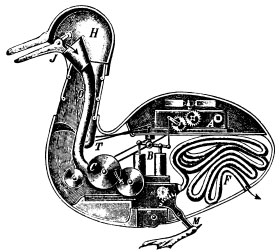
\includegraphics[scale=0.9]{Bilder/Duck_of_Vaucanson.jpg}			
	\caption{Vaucansons Ente}						
	\label{f:Ente}						
\end{figure}
Sodann wurden tatsächliche Automaten nur noch in sehr kleinen Formaten gebaut und diese waren auf Grund der hohen Fertigungskosten ausschließlich für wohlhabende Bürger vorbehalten. Deshalb wendeten sich die Techniker der Entwicklung von Nutzmaschinen zu, die durch die Erfindung von Dampf und Elektrizität als Antriebsmittel deutlich beschleunigt wurden. 

Die Idee Automaten zu bauen, die nützlichere Aufgaben erledigen sollten kam Anfang des 20. Jahrhunderts. So begann beispielsweise 1951 die Entwicklung ferngesteuerter Geräte zur Interaktion mit radioaktivem Material. 1954 wurde das erste Patent einer Roboterentwicklung durch den Briten C.W. Kenward eingereicht und 1959 der erste kommerzielle Roboter der Firma Planet Corp. vorgestellt. Dieser wurde mechanisch durch Kurvenscheiben und Begrenzungsschalter gesteuert. Ein erster mobiler Roboter (siehe Bild \ref{f:shakey}) wurde ca. 1968 am Stanford Research Institute entwickelt. Dieser war erstmals mit Sensoren, wie Kamera oder Tastsensoren ausgestattet.
\begin{figure}[H]						
	\centering							
	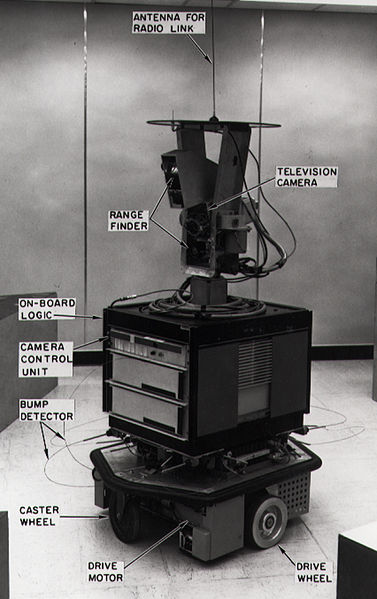
\includegraphics[scale=1]{Bilder/shakey.jpg}			
	\caption{Mobiler Roboter "`Shakey"'}						
	\label{f:shakey}						
\end{figure}
1978 wurde der Roboterarm PUMA\footnote{programmable universal machine for assembly, dt.: Programmierbare Universalmaschine für Montage - Anwendungen} vorgestellt. Er verfügte über einen elektrischen Antrieb und basierte auf Entwürfen von General Motors.
\\
\\
Zeitlich gesehen wird ab 1970 von Robotern gesprochen, da diese immer mehr mit ihrer Umgebung interagierten und nicht mehr "`starr"' ihre Bewegungen ausführten. Der Begriff Roboter oder mobiler Roboter wird im nächsten Abschnitt definiert.
 

\section{Definition}
Derzeit gibt es keine passende Definition, die den Begriff Robotik bzw. mobile Roboter so präzise formuliert, dass sie auf genau die Objekte passt, die nach gemeingültig einen Roboter definieren \cite{hertzberg2009mobile}. In \cite{hertzberg2009mobile} erklärt der Autor, dass es nicht unüblich ist, dass diese Unschärfe in der Definition großartig stört. Eine allgemeine Definition für Robotik ist in der \ac{VDI} Richtlinie 2860 von 1990 zu finden:
\\
\\
\textit{"`Ein Roboter ist ein frei und wiederprogrammierbarer, multifunktionaler Manipulator mit mindestens drei unabhängigen Achsen, um Materialien, Teile, Werkzeuge oder spezielle Geräte auf programmierten,
variablen Bahnen zu bewegen zur Erfüllung der verschiedensten Aufgaben."'}
\\
\\
Allerdings passt diese Definition nicht gut auf mobile Roboter. Diese Sprachregelung der \ac{VDI} zielt eher auf Handhabungsroboter aus der Automatisierungstechnik oder Kommissionierroboter aus dem Logistik - Bereich. Gemeint sind damit sogenannte \textit{stationäre Robotersysteme} \cite{Haun2007}. Diese sind starr mit der Umgebung verbunden und besitzen einen festgelegten Arbeitsraum. Damit sind die oben genannten "programmierten, variablen Bahnen" möglich, da der Arbeitsprozess in dem sich der Roboter befindet vorher bekannt und programmierbar ist. 

Mobile Robotersysteme unterscheiden sich zu stationären grundlegend, indem sie ihre Position durch Lokomotion (aus eigener Kraft) verändern \cite{Haun2007}. Somit hängen alle ihre Aktionen direkt von ihrer aktuellen Umgebung ab, die detailliert immer erst zum Zeitpunkt der Ausführung bekannt wird \cite{hertzberg2009mobile}. Sowohl \cite{hertzberg2009mobile} als auch \cite{Haun2007} heben die Eigenschaft hervor, dass mobile Roboter ihre Umgebung mittels Sensoren erfassen und auswerten müssen. Aus dem Ergebnis der Auswertung wählen sie schließlich ihre nächste Aktion. Ferner werden in \cite{Haun2007} folgende, weitere Eingeschaften genannt:
\begin{itemize}
\item aufgabenorientierte und implizierte Programmierung
\item Anpassung an Veränderungen an die Umgebung
\item Lernen aus Erfahrungen und entsprechende Verhaltensmodifikation
\item Entwicklung eines internen Weltbildes
\item Manipulation physikalischer Objekte in der realen Welt
\end{itemize}
Das bedeutet im Allgemeinen, dass ein mobiler Roboter in einer zuvor nicht bekannten und nicht kontrollierbaren Umgebung zu jeder Situation umgebungsabhängig operieren muss. Im Vergleich zu stationären Robotern bedeutet dass nicht, dass die mobilen Roboter Regellos oder zufällig arbeiten, die entsprechenden Anweisungen sind "`weicher"', wie zum Beispiel eine Bahnplanung eines Industrieroboters.

Mit welchen internen und externen Sensoren ein Roboter seine Umgebung verarbeitet, wird in Kapitel \myref{Komponenten} erklärt.


\subsection{Roboterarten}
Die \textbf{Serviceroboter} sind Maschinen, die den Menschen bei der täglichen Arbeit unterstützen sollen. Darüber hinaus sollen sie auch in der Lage sein als Unterhaltungssystem zu dienen. Es wird geschätzt, dass in ca. 30 Jahren mehr persönlicher Roboter produziert werden als persönliche Computer \cite{Haun2007}.
Diese sollten am Besten auf Zuruf alltägliche Arbeit erledigen. Dazu zählt Staub saugen, Rasen mähen oder auch Fenster putzen. Dabei tritt häufig ein zentrales Problem in den Vordergrund: die Anatomie des Menschen. Diese ist ein regelrechtes Wunderwerk, da beispielsweise die menschliche Hand bei einem durchschnittlichen Gewicht von 600 Gramm und 23 verschiedenen Freiheitsgraden dazu in der Lage ist, Bewegungen mit stufenlos verstellbarer Feinfühligkeit durchzuführen. Vor allem japanische Forscher stecken viel Arbeit in die Erforschung immer besser werdender Serviceroboter. Der durch Honda im Jahr 2001 vorgestellte Serviceroboter \textit{Asimo} ist bei einer Größe von 1.20 Meter nur noch 43kg schwer (siehe Abbildung \ref{f:asimo}).
Dabei ist eine der größten Herausforderungen die Stromversorgung. Ein Roboter der ständig am Ladegerät hängen muss, hilft dem Menschen nicht weiter. Daraus resultiert, dass kommerzielle Anbieter von Staubsaugrobotern Räder als Antrieb benutzen. Dies Roboter müssen ihre Bewegungen nicht ständig korrigieren. Sie fahren in konstanter Bodennähe durch die Gegend. Ferner ist die Interaktion zwischen Roboter und Mensch ein Problem. Das Robotersystem muss Daten nicht nur messe und analysieren, sondern auch bewerten können. Dabei gibt es immer noch keine geeignete Verarbeitung der intuitiven Kommunikation, die beim Menschen über Gestik, Mimik und Sprache erfolgt. So wird es noch ein paar Jahre dauern, bis Serviceroboter uns wirklich im Alltag unterstützen können.
\begin{figure}[H]						
	\centering							
	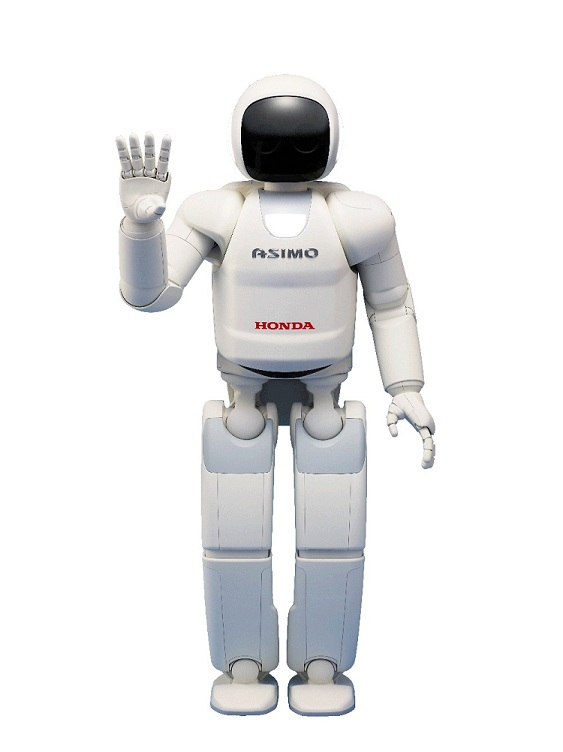
\includegraphics[scale=0.5]{Bilder/asimo.jpg}			
	\caption{Roboter ASIMO}						
	\label{f:asimo}						
\end{figure}

\textbf{Industrieroboter} hingegen haben sich in der aktuellen Zeit schon sehr etabliert. VW setzt an einen Produktionsstandort ca. 760 Industrieroboter ein und in Deutschland sind es sogar mehr als 100.000 \cite{Haun2007}. Im Gegensatz zu den Servicerobotern haben sie meist nur einen Arm und besitzen keine Beine und keinen Kopf. Ihre Aufgabe besteht darin selbst tonnenschwere Lasten zu heben und pausenlos gefährliche Arbeit wie z.B. Schweißen durchzuführen. 
Theoretisch kann jedes Fertigungsproblem heutzutage auch maschinell gelöst werden. In der Autoindustrie gibt es beispielsweise weite Bereiche (Herstellung Karosserie), wo Roboter dominieren. Dafür zeigt sich in der Endmontage, dass Roboter deutlich in der Minderheit sind. Zukünftig werden die Industrieroboter statt umständlich und in komplizierten Sprachen über eine grafische Benutzeroberfläche verfügen und ihre Aufgaben per Sprachsteuerung erklärt bekommen \cite{Haun2007}.

Robotersystem werden auch im Bereich der \textbf{Medizin} eingesetzt. Durch ihre Präzision fräsen sie beispielsweise Hüftgelenke so exakt aus, dass die Ersatzteile nahtlos und ohne Zement eingefügt werden können. Die Vorteile sind, dass sie frei von emotionalen Einflüssen sind und keine Tagesform kenne. Egal zu welchem Zeitpunkt, die programmierte Aufgabe erledigt der Roboter immer gleich. Jedoch sind sie teuer und kompliziert. Die Operation muss im Vorfeld genauestens geplant werden und auf sich plötzlich verändernde Gegebenheiten kann ein Automat nicht reagieren. So musste unter anderem der \textit{Robodoc} abgeschaltet werden, da er Menschen Schaden zugefügt hat. Dadurch hat sich derzeit der Einsatz von Robotern in der Medizin eher auf die Form eines Assistenten reduziert. Die Maschine hält dabei Skalpell und Nadel und führt als verlängerter Arm aus, was der menschliche Operateur hinter dem Steuer vorgibt \cite{Haun2007}. Solche System werden vor allem bei Herzoperationen eingesetzt, da sie jedes Zittern des Menschen herausfiltern und so an kleinsten Gefäßen und Strukturen arbeiten können. Die Roboter helfen dabei, schwierige Operationen einfacher zu machen.

\textbf{Humanoide Roboter} sind menschenähnliche Roboter wie \textit{Asimo} (Abbildung \ref{f:asimo})oder Nao. Ihr Bau ist nicht nur durch den Spieltrieb der Robotiker oder der Sensationslust des Publikums motiviert. Auch wissenschaftliche Aspekte sprechen für den Bau humanoider Roboter. So wird nur ein Roboter mit einem menschenähnlichen Körper auch menschenähnliche Begriffe und Denkweisen entwickeln (Johnson 1987). Ferner spielt natürlich auch der psychologische Aspekt im Bereich der Servicerobotik eine Rolle. Wenn etwas wie ein Mensch aussieht, wird damit auch umgegangen wie mit einem Menschen. Einem humanoiden Roboter kann ein Mensch, wie seinem menschlichen Gegenüber, seine Wünsche mitteilen und braucht dafür keine Gebrauchsanweisung. Dazu kommt, dass ihre Körper auch auf die Umgebung abgestimmt sind, in der sich der Mensch bewegt.



\section{Komponenten}\label{Komponenten}

\section{Freiheitsgrad}
Der Begriff Freiheitsgrad oder DOF (engl.: Degree(s) of Freedom) bezeichnet die Zahl voneinander unabhängigen Bewegungsmöglichkeiten eines Systems. Ein starrer Körper im Raum hat beispielsweise einen Freiheitsgrad von sechs. Er kann sich in drei voneinander unabhängigen Richtungen bewegen und in drei voneinander unabhängigen Ebenen drehen. Als \textit{Freiheiten} werden dann die einzelnen Bewegungs- bzw. Rotationsmöglichkeiten bezeichnet. Somit hat der starre Körper je drei Translationsfreiheitsgrade und Rotationsfreiheitsgrade. 

\cite{hertzberg2009mobile} definiert Freiheitsgrad in zwei Ausprägungen: 
\begin{itemize}
\item Aktiver Freiheitsgrad bezeichnet die Zahl der translatorischen wie rotatorischen Bewegungen, die eine Gelenk oder eine Roboterkomponente ausführen kann. Dies deckt sich also mit der Definition von oben.
\item Effektiver Freiheitsgrad bezieht sich auf die \textit{Pose}. Sprich die Dimensionierung der Position und Orientierung, die ein Roboter einnehmen kann.
\end{itemize}
So hat beispielsweise ein differentialgetriebener Roboter, der sich nur in einer Ebene bewegen kann zwei aktive, dagegen aber drei effektive Freiheitsgrade.

Wenn ein Robotersystem direkt von jeder möglichen Pose in jede andere mögliche Pose wechseln kann, wird von einem \textit{holonomen} Robotersystem gesprochen. Solche Roboter sind beispielsweise diejenigen, die in der Lage sind in jede beliebige Richtung zu fahren, ohne davor eine Drehung machen zu müssen. Als allgemeine Regel gilt: \\
$ nicht-holonom = DOF_{effektiv} > DOF_{aktiv} $ \\
Das heißt, ein System ist auf jeden Fall nicht holonom, wenn die Anzahl der effektiven Freiheitsgrade größer wie die der aktiven ist.